%
%        Document : Megabolt : Cross Platform Download Manager.Project report
%        Author   : Arjun S R
%        Date     : Thu Apr  7 18:15:04 IST 2011

\documentclass[pdftex,12pt,a4paper,pdfencoding=unicode]{article}
\usepackage[pdftex]{graphicx}
%\usepackage[dvips, bookmarks, colorlinks=false,pdftitle={Megabolt},pdfauthor={Arjun S R},pdfsubject={Project Report},pdfkeywords={PDF, LaTeX, hyperlinks, hyperref}]{hyperref}

\usepackage{hyperref}
\usepackage[all]{hypcap}
\usepackage{amstext}
\usepackage{setspace}
\usepackage{tabularx}
\usepackage{multirow}
\usepackage[english]{babel}
\usepackage{fancyhdr}
\usepackage{fixltx2e}
\usepackage{color}
\usepackage{xcolor}
\usepackage{parskip}
\usepackage{bookmark}
\usepackage{cite}
\usepackage[a4paper]{geometry}
\usepackage{float}
\usepackage{rotfloat}
\usepackage[T1]{fontenc}

% should uncomment line below only if the document is to be compiled to times new roman font
%\usepackge{times}

\DeclareGraphicsExtensions{.pdf,.png,.jpg,.jpeg}
\newcommand{\HRule}{\rule {\linewidth}{0.5mm}}
\newcommand{\CRule}{\rule {\linewidth}{0.78975mm}}

\setcounter{tocdepth}{4}
\setlength{\parindent}{1cm}
\setcounter{table}{0}

\begin{document}
\begin{titlepage}
  \begin{center}
    {\huge \bfseries Megabolt : Cross Platform Download Manager}\\[1cm]
    \textsc{\large Project Report}\\[7.5mm]
           {\large \it Submitted in partial fulfillment of the requirements\\ for the award of the
             Degree of Bachelor of Technology\\ in Computer Science \& Engineering\\ of the University of Kerala}
           \begin{center}
             \large
             \centering
             \emph{ By}\\ \vspace{1mm}
                  {\bf Arjun \textsc{S R} }\\ \vspace{1mm}
                  {\bf Deepak Kumar \textsc{N D}}\\ \vspace{1mm}
                  {\bf Joji Antony}\\ \vspace{1mm}
                  {\bf Sreekanth Balakrishnan}\\ \vspace{1mm}
                  {\bf Varun \textsc{V V}}\\ \vspace{1mm}
                  
\includegraphics[scale=0.90]{pic/cetemblem.jpg}
           \end{center}
               {\textsc \bf \large Department of Computer Science and Engineering\\ College of Engineering\\ Trivandrum\\ 2011 }
  \end{center}
\end{titlepage}


\hypersetup{
  bookmarks=false,          % show bookmarks bar?
  unicode=true,             % non-Latin characters in Acrobat’s bookmarks
  pdftoolbar=true,          % show Acrobat’s toolbar?
  pdfmenubar=true,          % show Acrobat’s menu?
  pdffitwindow=true,        % window fit to page when opened
  pdfstartview={FitH},      % fits the width of the page to the window
  pdftitle={Megabolt},      % title
  pdfauthor={Arjun.S.R},    % author
  pdfsubject={Megabolt:A Cross-Platform Download Manager},   % subject of the document
  pdfcreator={Arjun.S.R},   % creator of the document
  pdfproducer={Arjun S.R}, % producer of the document
  pdfkeywords={megabolt} {free} {download manger}{cross-platform}, % list of keywords
  pdfnewwindow=true,      % links in new window
  colorlinks=true,       % false: boxed links; true: colored links
  linkcolor=red,         % color of internal links
  citecolor=green,       % color of links to bibliography
  filecolor=magenta,      % color of file links
  urlcolor=cyan         % color of external links
}


\begin{onehalfspace}
  \section*{}
  \thispagestyle{empty}
  \begin{center}
    {\large \bf DEPARTMENT OF COMPUTER SCIENCE AND ENGINEERING}\\
    {\small \bf COLLEGE OF ENGINEERING}\\
    {\small \bf TRIVANDRUM}\\
    {\small 2011}\\
    \vspace{5mm}
    
\includegraphics[scale=0.75]{pic/cetemblem.jpg}\\
                    {\large \bf CERTIFICATE}\\[0.75cm]
  \end{center}
      {\it This is to certify that this project entitled {\textsc MEGABOLT - A CROSS PLATFORM DOWNLOAD MANAGER}
        is a bonafide record of the project done by {\bf \emph{Arjun.S.R, Deepak Kumar.N.D, Joji Antony, Sreekanth B,}}
        and {\bf \emph{Varun V.V}} under our guidance \& supervision towards the partial fulfillment of the requirements
        for the award of the Degree of Bachelor of Technology in Computer Science and Engineering of the University of
        Kerala during the year 2010-2011.}

      \begin{minipage}{0.4\textwidth}
        \begin{flushleft}
          {
            \small \emph{Project Guide}\\
                   {\bf Mrs.Deepthi V R,}\\
                   Lecturer,\\
                   Dept of CS \& Engg,\\
                   College of Engineering,\\Trivandrum
          }
        \end{flushleft}
      \end{minipage}
      \begin{minipage}{0.4\textwidth}
        \begin{flushright}
          {
            \small
            \emph{Project Coordinator}\\
                 {\bf Prof.Shreelekshmi R,}\\
                 Head Of the Department\\
                 Dept of CS \& Engg,\\
                 College of Engineering,\\Trivandrum
          }
        \end{flushright}
      \end{minipage}
      \vfill
      \newpage
      \section*{}
      \thispagestyle{empty}
      \begin{center}
        {\bf ACKNOWLEDGEMENT}
      \end{center}
      We wish to place on record our deep sense of gratitude to our project guide, {\bf Mrs.Deepthi V R}, Lecturer, Department
      of Computer Science \& Engineering, College of Engineering, Trivandrum, for most valuable help and support in carrying out this
      preliminary project work and also for her concern shown during intricate situations.\\

      \indent We hereby express our sincere thanks to {\bf Mrs. Shreelekshmi R}, Head of the Department, Department of Computer
      Science \& Engineering, College of Engineering, Trivandrum for all the necessary help extended during the course of the work.\\

      \indent We would also like to extend our sincere thanks to all staff members of the Department of Computer Science \&
      Engineering, College of Engineering, Trivandrum whose help has led to the completion of this report.\\[1cm]
      \begin{minipage}{0.4\textwidth}
        \begin{flushleft}
          {
          }
        \end{flushleft}
      \end{minipage}
      \begin{minipage}{0.4\textwidth}
        \begin{flushright}
          {
            \emph{Arjun.S.R\\Deepak Kumar.N.D\\ Joji Antony\\ Sreekanth B\\ Varun V.V\\}
          }
        \end{flushright}
      \end{minipage}
      \vfill
      \newpage

      \section*{\Large Abstract}
      \thispagestyle{plain}
      Megabolt is cross-platform download manger written in Qt Framework with many interesting features
      capable of professional use. Megabolt uses threaded downloaded on all the protocols it supports.
      The software is released in BSD licensed.\\

      Our project was mainly intended to write portable code that runs light-weight processes on various
      platforms that Qt supports and provides a simple front-end to initiate, configure and use the software.
      Extra care was given in making the software configurable. The data structures are generic that supports
      almost all file transfer protocols available right now in the industry.

      \newpage
      \begingroup
      \hypersetup{linkcolor=blue}
      \tableofcontents
      \endgroup
      \thispagestyle{empty}
      \newpage
      \listoffigures
      \thispagestyle{empty}
      \newpage
      \pagestyle{fancy}
      \fancyhead[R]{\leftmark}
      \fancyhead[L]{\rightmark}
      \fancyfoot[C]{\thepage}
      \section{Introduction}
      \setcounter{page}{1}
      At this point of the century, internet is the largest source of data and file. When data holds something that is useful; the
      data becomes information. Most of the worlds population uses internet for searching information and downloading files etc.
      And there arises the need of a well architectured, designed and friendly download manager. Computer networks as designed,
      the data is sent in the form of packets through various intervening routers and proxies.

      A download manager is a software that are usually tailored to automate downloads of various files hosted in the internet. The
      protocols with which the files may be shared may be HTTP, HTTPS, FTP, SFTP, metalink or even cookie based connections. So it means
      that we need a download manager that extends its service to operate over the above protocols and function efficiently. So we went
      on with the idea of making one. But, after that we realized that the coding phase is going to be hectic. We, the developers of the
      software wanted the software to be free in all its means because that is the only way to provide something best to the society to
      solve a common problem. A more close look at the networking API of the modern system made it clear that the thread management is
      different for different operating systems. Moreover the TCP/IP kernel stack is different from each other with incompatible extension
      and methods.

      We needed a single code base that can be used to run in all the environments. Such thoughts made us to think of even using scripting
      languages like python or perl for the software. Later, we got in touch with Nokia's Qt. Qt is widely used in many projects. Qt is a
      extended C++ language. It has a middle interfacing template layer that interfaces all the devices and jobs that are very abstract and
      generic; which gives the developer the freedom to use or even re-implement the functions to adapt to its requirements in the software.
      Qt code when compiled the host operating system passes some of its properties and environment variables that the Qt uses to make the
      code work on its platform. Our code runs straightaway in platforms like GNU/Linux, M S Windows and Apple MAC OSX kernels (more kernels
      to be experimented).

      \subsection{Basic Operation of a Download Manager}
      Download manager functions can be split in to various layers:
      \begin{description}
      \item[Front End :] The download manager has a very lightweight, easy and simple front end. The main purpose of the front end is to
        insert \emph{download items} or \emph{uri's} to the object to be downloaded. Helps in entering the scheduling information.
        Front provides the service to configure the internal parameters of the download manager. Special effort was given in making the
        user interface simple because well verbose and crowded sophisticated can ward off naive users.

        There are cases in which the protocol demands user or login credentials to login and download, here the download managers front
        helps in getting it from the user and automating it. Front ends provides a search bar that helps the user to search his/her
        download with the name in the list. All the downloads are put in a list, based on the status the object are created else its
        just read in to fill the list.

      \item[Manager :] Manager is the heart of the download manager. Manager by virtue of its name has a lot of responsibilities. The
        manager reads the list of download \emph{uri's} and fills the list. If the download is not finished, it initiates the download
        objects. Manager check the \emph{maximum number of concurrent downloads} configured and initiates that much number of downloads
        through the virtual  function \emph{start()}. Manger frequently checks the status and provides feedback through the progress bar
        regarding the percentage of the download. \emph{Scheduler} plays a very important role in managing the task in the list. Object
        in the list can have a global scheduler that acts on a whole to the list. But if you feel like doing some scheduling specific
        to a file a local scheduling is provided to initiate at a particular point of time.

      \item[Back End :] Back end includes the real protocol dependent layer. Each protocol have there own specific details and extra
        files to be handled. The layers were well designed so that each layer can function independently without much sharing of datas.
        The interfacing API in the \emph{front end} is generic so that it can act on object of various protocols. The back end deals with
        connecting to the server with details given from the front end including user credentials, number of connections per download,
        destination file to write the data, thread status metadata, timing information to implement throttling of the download.
      \end{description}

      \subsection{Project Description}
      Download manager is a specialized software that is capable of handling downloads given to it transparently in a self-contained
      way. Download manager identifies the type of the file being downloaded and makes proper destined download directories so that
      all the files that are downloaded will be well organized as per the media type. Irrespective of where the download manager runs,
      it has to provide support to download through firewall and proxies. The download manager has following properties:
      \begin{itemize}
      \item It is cross platform. Work on popular kernels like GNU/Linux, MS Windows and MAC OSX\ldots. Also on all platforms where Qt runs
      \item Ability to configure individual download
      \item Threaded download support
      \item Extensible code, so its easy to write modules for newer protocols
      \end{itemize}
      \newpage
      \section{Field of research}
      Most of the current download manager just provide a mechanism to download and a simple automation of downloads by allowing batch
      scripts and cron jobs. Many download managers and download accelerators in the market where studied so as to make our software
      fool proof and the best in the market.

      \subsection{Background of research}
      Download managers in the market are generally platform specific. Some may be good in threaded support but may be bad in other feature.
      So the market really lacked a well generically defined and designed download manager that can be configured in the native OS to run
      conflict less. Download managers attached to the browser cannot function independently.They need the browser's framework to carryout
      its function. Download managers like IDM, orbit, axel, aria2c, free download manager, downthemall(addon to firefox) were all studied.

      Internet users first wanted to stream movies and download basic mp3 files. Later after broadband connection they demanded high
      definition videos. And with 3G they started demanding blu-ray videos, HDTV live stream and so on. So the need to download data
      just increases the way the field of networking and multimedia advances.

      Many internet service providers issues offer in free download time of the least traffic in their timezone. Some users find it really
      difficult to exploit this chance as it is hard to change their routines to this free download time. So a mechanism to automate or
      schedule download was noted.

      Most of the servers today provide downloads through HTTP, FTP, HTTPS, session based download and cookie based download. A detailed
      study of the HTTP[RFC 2616] and FTP [RFC 959] were made to implement it in the project. To cut it short and make the coding faster
      we first implemented  HTTP downloads.

      \subsection{Problem Definition}
      As we all know the popular operating systems include GNU/Linux, M S Windows, Apple's MAC etc\ldots. In each kernel the internal
      implementation of the networking application programming interface is entirely different. Though the networking API in linux is
      compatible with BSD socket interface. There are many internal issues that make it different from each other.

      The graphical user interface library for windows is a part  WIN32 api entirely different from Apple's Cocoa ; which again is totally
      different from *nix based X Window systems.

      As the OS kernel's differs so does the abstraction for a process in the system as well as the way OS treat its user space threads are
      usually very specific. M S Windows in its thread and process based syscalls the internal implementations are not much POSIX compliant
      which makes the task more difficult.

      The way each system handles the file streams are too different. The formatting scheme they follow are confliciting adding to the above
      problems making it more tougher to think of code portability.

      After making out all the issues that we faced in researching about the download managers in the market we got the idea that we should
      use a language that is platform independent, efficient, lightweight and very maintainable. Many choices were there like JAVA which
      will make the working of the code more safer in the JVM and portability was assured inherently. But we wanted more efficiency and
      increase in the performance. Later thought of using scripting languages like python and perl which would make the code execute on
      almost all platforms and the lines of code will be considerably less but had to tradeoff efficiency.

      Then we came across the extended grammar form of the language C++ that is called \emph{Qt}. Its a programming language.
      That is it when compiled produces a binary
      \begin{enumerate}
        \item That runs on the native operating system without any other interpreter. -efficiency.
        \item It gives precise control on the thread management facility offered by the system. -portability of threads
        \item It gives more neat code - maintainability.
        \item It gives a intermediate layer that interface various devices, networks of various operating systems.
          -portability of networking API.
        \item It gives a intermediate layer that interface various graphical user interface libraries of operating systems
          to be compiled to the platform. -portability of gui code.
      \end{enumerate}

      \subsection{Summary of research}
      The research on the field of application level protocols and other operating system internals helped us to make our design simple and
      elegant. The software will provide the features described below :
      The software is simple which initializes its parameters by its configuration file. Reads through the set of links to downloads stored
      in pre-defined directory which contains details to its scheduling information, throttling information, thread status information and
      details of the file to be download like destination directory etc\ldots

      Design was very sophisticated that makes the backend completely independent with a layered architecture. Backend can function
      independently as a command-line downloader like \emph{wget} however scheduling and other details have to be either hand coded to
      the configuration files or as command-line arguments.

      \subsubsection{Solution Overview}
      Our portable download manager has only a single code that compiles in almost all major OS platforms. When compiled it link the
      native GUI API calls to get things done. The code is compiled to the networking module of the native platform. Which makes it
      whole new faster product. Also Qt 4 was re-written for make it faster and efficient as it was getting heavy.

      The basic algorithm is like this, when the software is run ; it initializes it with predefined files that contain various directory
      paths. The list of url's to be downloaded is read. The status is checked. If not completed the download object is initialized and
      started by calling a virtual function \emph{start()} and it can be paused using \emph{pause()} function. The socket function within
      these functions are non-blocking. Scheduling can be performed either list wise or individual file wise. If individual scheduling is
      specified it overrides the list wise global scheduling information.

      The main thread in the backend makes a timeout of 300milli second so as to write back the data it received till that slice to the
      disc and it updates the thread status which makes the download pause resumable.

      The software is released in GPLv3 which makes the code completely \emph{free} and open to contribute. If there is a way to provide
      a good solution to layman's needs in software; it is to make the code \emph{free}. The data structures that are used in the project
      which will be discussed in next section is generic and extensible. Its really add support to another protocol class.
      \newpage
      \section{Project Modules and Description}
       Download manager is a software that manages, schedules, accelerates and automate downloads. Its a widely software nowadays. However,
       such an open, cross-platform with so much features are not available in the download managers currently available in the market.

       Various modules included in the project are :
       \begin{enumerate}
       \item Front end : The front end includes scrollbars, stringlists, resizers, buttons, checkboxes, calendars and many widgets from
         the Qt framework that helps to build the basic graphical user interface. Its description here is out of scope of the project
         report.
       \item Manager : Manager is the core module that instantiates all other modules in the download manager. Software once started
         takes parameters from the operating system and initializes it configuration file directories. With configuration files it reads the
         user preferences and settings.

         Manager reads the list of download \emph{uri's} checks its status in the metadata. Object is passed to the backend if unfinished to
         instantiate the protocol dependent download class. A download of an object is initialized by calling a \emph{start()} virtual
         function.

         Manager has the responsibility to check the scheduling information regarding a download object and call it timely. Manager
         processes ``maximum concurrent number of downloads'' and the backend replies frequently updating its progress. This is shown
         at the progress bar to give continous feed back to the user. The manager initializes the object with respect to the scheme entry
         in their urls.

       \item Back end : The back end is the core protocol specific part the does the task of downloading. All the data need the back end
         is provided by the manager. Manager have only \emph{start()} and \emph{pause()} actions on the backend subsystems. The preliminary
         model of the project has only implemented basic HTTP [RFC 2616] downloads.
       \end{enumerate}
       \newpage
       \section{Specification and Design}
       As the project is named as cross-platform download manager considerable effort was made to not to include non-portable code.
       Unlike other download managers, megabolt downloads through various thread and writes it to the same file than downloading it into
       parts and joining it in the future. That causes useless computation while joining the file and there is a need to have considerable
       memory and disk space usage during the joining of the files. To avoid this we put a semaphore for writing to the files concerned.

       Megabolt has following features:
       \begin{itemize}
       \item It is a free software. Free as in freedom.
       \item It is cross platform. It works on majority of the popular OS like GNU/Linux, Apple's MAC OSX and M S Windows\ldots
       \item It support threaded download support. As we all know a single TCP/IP connection for the transfer for a file is very
         obselete and the connection cannot fully exploit the capacity of the transmission medium beyond a limits due to the threshold
         limits with just one connection. To use the complete channel bandwidth we use multiple connections for a single file which
         makes download faster and better.
       \item Scheduled downloads are possible. Scheduling our job is one of the most important task.
       \item HTTP following is implemented.
       \item Pause resume support is implemented.
       \item Provides mechanism to throttle the connection made for a file. If you want that the download you make shouldnt hog up
         the network bandwidth beyond a particular limit you can configure it.
       \item Simple graphical user interface design.
       \end{itemize}

       Beyond all, megabolt provides a abstract way of making download manager.

       \subsection{Front end}
       The data structures are generic that aids to write
       extensible code to add more protocol support. 
       \begin{figure}[h!]
         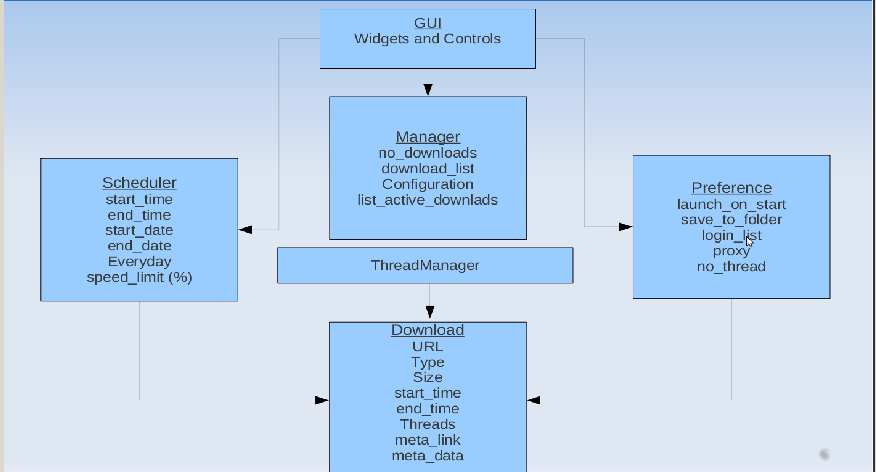
\includegraphics[scale=0.50]{pic/hier.png}
         \caption{Class hierarchy \label{fig:hier}}
       \end{figure}
       For more details check the Figure : Class hierarchy\ref{fig:hier}
       Above diagram shows the main classes involved in the project. Now next figure shows you the methods and the control flow in the 
       classes.

       \subsection{Manager}
       This the core module that  has control over the backend. This modules give a time slice like 200 millisecond and update the status
       of the individual download object. It functions in a multi-threaded fashion in order to serve \emph{ max concurrent downloads } of
       objects and to update each one's status. Check figure \ref{fig:methods}
       \begin{figure}[h!]
         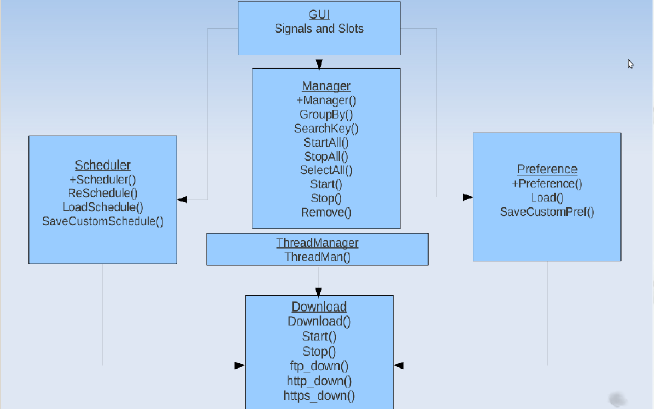
\includegraphics[scale=0.90]{pic/methods.png}
         \caption{Member functions of various classes \label{fig:methods}}
       \end{figure}

       \subsection{Backend}

       Only HTTP downloads were implemented in the preliminary phase. The HTTP threads behave according to the following finite state
       automaton\ref{fig:ts}. This module functions in a multi-threaded fashion. The main thread resolves the links to follow it until
       actual location is obtained. The main thread frames requests as per standard HTTP format. The main thread spawns of mentioned
       number of worker threads. These worker threads frequently writeback the buffer full of data to the disk based on a timeout.
       \newpage
       \begin{figure}[h!]
        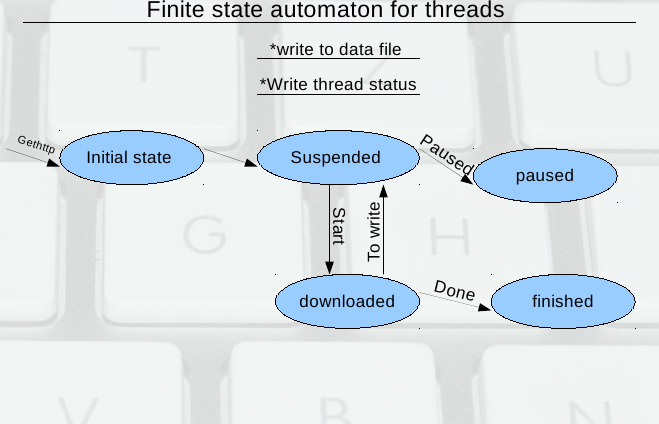
\includegraphics[scale=0.90]{pic/ts.png}
         \caption{Finite State Automaton of a single thread \label{fig:ts}}
       \end{figure}

       The finite state automaton of the thread is shown above. After the 300 millisecond timeout each thread goes to suspended state.
       In the suspended state the thread seeks to the range based position in the file and write it data downloaded and updates its thread
       status information in the metadata file.

       \newpage
       \section{System Configuration}
       \subsection{Hardware Configuration}
       \begin{description}
         \item[Processor :] Intel Pentium 3 or above
         \item[RAM :] 256MB or above
         \item[HDD: ] 40 GB
       \end{description}

       \subsection{Software Requirements}
       \begin{description}
       \item[ Operating system ]: Any (Megabolt is Portable!)
       \item[ Development Tools]: Qt Creator 4 and Qt Designer
       \item[Version control] : Git
       \end{description}
       \newpage
       \section{Screen shots}
       Adding URL \ref{fig:ss2}
       \begin{figure}[h!]
         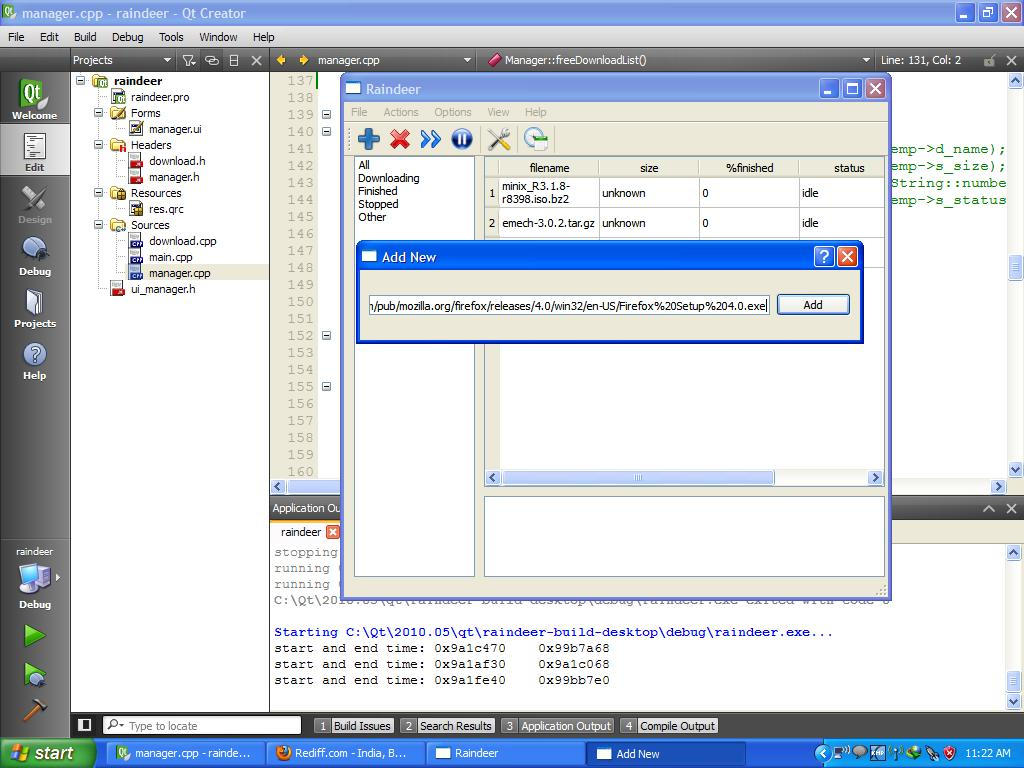
\includegraphics[scale=0.60]{pic/ss2.jpg}
         \caption{Screenshot \label{fig:ss2}}
       \end{figure}
       \newpage
       \section{Conclusion and Future Works}
       We intend to increase performance and do more work on this project on various areas.
       \begin{itemize}
       \item We intend to study the optimal buffer size that needs to given with the thread by studying the network output through
         simulation tools like \emph{ dummy network}. By statistical analysis of packet loss rate and bandwidth we intend to deduce an
         optimal buffer size for the download threads so that in the time slice the buffer wont filled in a burst also the minimizing
         the non-filled portion of the buffer.
       \item Add protocol support for FTP, HTTPS and session based downloads.
       \item Right now we have support only for caching proxy. Support needs to give to more proxies.
       \item Integrate megabolt with major browsers like Google chrome, Mozilla Firefox etc aby creating an addon to megabolt.
       \item Code is ready for release in GPL to the community.
       \end{itemize}
       
       We had a really good learning experiend doing this project and also found many core papers like theory of computation, computer
       networks and other core papers were really worth learning.
       
       \newpage
       \section*{Bibliography}
                {\bf [1] Fielding.et.al RFC 2616 HTTP}\\ \href{http://tools.ietf.org/html/rfc2616}\\
                {\bf [2] RFC 959 FTP} \\ \href {http://tools.ietf.org/html/rfc959}\\
                {\bf [3] The Open Group Base Specifications IEEE Std 1003.1}\\
                {\bf [4] Qt Documentation}\\ \href{http://doc.qt.nokia.com/latest/}\\
                
                \addcontentsline{toc}{section}{Bibliography}
\end{onehalfspace}
\end{document}
